\section{Results}
\subsection{Minikube results}
After running the commands in Listings~\ref{lst:minikube-cluster}, the Minikube creates a three-node cluster with two worker nodes and one control plane node.
This is shown in Figure~\ref{fig:minikube-cluster}.

\begin{figure}[htbp]
  \centering
  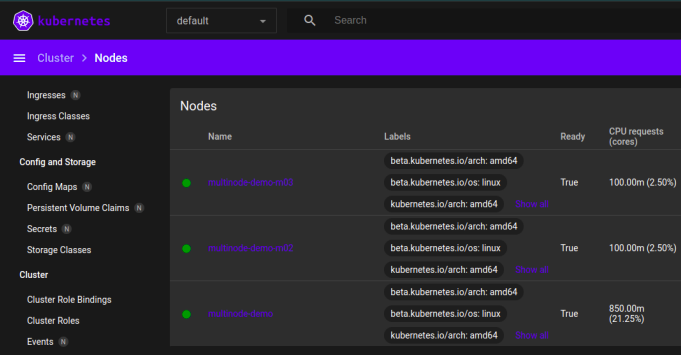
\includegraphics[width=0.45\textwidth]{figures/nodes.png}
  \caption{Minikube cluster with three nodes.}
  \label{fig:minikube-cluster}
\end{figure}

After running the commands in Listings~\ref{lst:kubectl_php_apache}, the PHP Apache server is deployed on the Minikube cluster.
The dashboard shows the deployment and service created, as shown in Figure~\ref{fig:deployments} and Figure~\ref{fig:services}, respectively.

\begin{figure}[htbp]
  \centering
  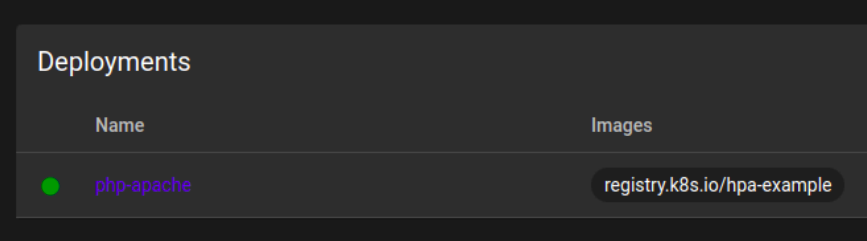
\includegraphics[width=0.45\textwidth]{figures/deployments.png}
  \caption{PHP Apache server deployment.}
  \label{fig:deployments}
\end{figure}

\begin{figure}[htbp]
  \centering
  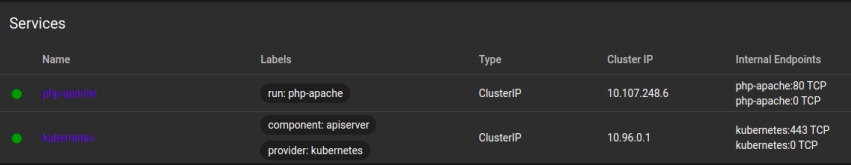
\includegraphics[width=0.45\textwidth]{figures/services.png}
  \caption{PHP Apache server service.}
  \label{fig:services}
\end{figure}

\subsection{AWS EKS results}
